\documentclass{standalone}

\usepackage{tikz}
\usepackage{standalone}

\usetikzlibrary{arrows,positioning, decorations.pathreplacing, calc, backgrounds}
\tikzset{
    ncbar angle/.initial=90,
    ncbar/.style={
        to path=(\tikztostart)
        -- ($(\tikztostart)!#1!\pgfkeysvalueof{/tikz/ncbar angle}:(\tikztotarget)$)
        -- ($(\tikztotarget)!($(\tikztostart)!#1!\pgfkeysvalueof{/tikz/ncbar angle}:(\tikztotarget)$)!\pgfkeysvalueof{/tikz/ncbar angle}:(\tikztostart)$)
        -- (\tikztotarget)
    },
    ncbar/.default=0.5cm,
}
\tikzset{square left brace/.style={ncbar=0.5cm}}
\tikzset{square right brace/.style={ncbar=-0.5cm}}

\begin{document}
    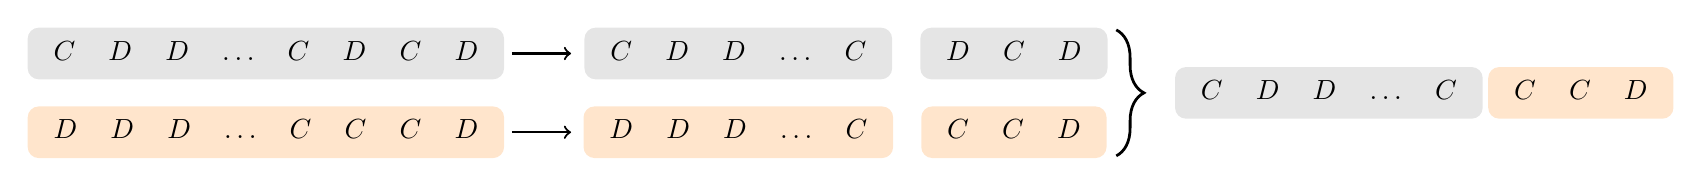
\begin{tikzpicture}
        % \node (n) at (0, 0) {\footnotesize \(N=205\)};
        \node[rectangle, fill=gray!20, rounded corners] (parent_one) at (0, 0) {\begin{tabular}{ccccccccc}
            \(C\) & \(D\) & \(D\) & \(\dots\) & \(C\) & \(D\) & \(C\) & \(D\) \\
            \end{tabular}};
        \node[rectangle, fill=orange!20, rounded corners] (parent_two) at (0, -1) {\begin{tabular}{ccccccccc}
            \(D\) & \(D\) & \(D\) & \(\dots\) & \(C\) & \(C\) & \(C\) & \(D\) \\
            \end{tabular}};

    \node (in) at ($(parent_one)+(3, 0)$) {};
    \node (out) at ($(parent_one)+(4, 0)$) {};
    \draw (in) edge[out=0, in=180, ->, thick] node {} (out);
    \node (in) at ($(parent_two)+(3, 0)$) {};
    \node (out) at ($(parent_two)+(4, 0)$) {};
    \draw (in) edge[out=0, in=180, ->, thick] node {} (out);

    \node[rectangle, fill=gray!20, rounded corners] (part_one_parent_one) at ($(parent_one)+(6, 0)$) {\begin{tabular}{ccccc}
        \(C\) & \(D\) & \(D\) & \(\dots\) & \(C\) \\
        \end{tabular}};
    \node[rectangle, fill=gray!20, rounded corners] (part_two_parent_one) at ($(parent_one)+(9.5, 0)$) {\begin{tabular}{ccc}
            \(D\) & \(C\) & \(D\) \\
            \end{tabular}};

    \node[rectangle, fill=orange!20, rounded corners] (part_one_parent_two) at ($(parent_two)+(6.0, 0)$) {\begin{tabular}{ccccc}
        \(D\) & \(D\) & \(D\) & \(\dots\) & \(C\) \\
                \end{tabular}};
    \node[rectangle, fill=orange!20, rounded corners] (part_two_parent_two) at ($(parent_two)+(9.5, 0)$) {\begin{tabular}{ccc}
        \(C\) & \(C\) & \(D\) \\
                    \end{tabular}};

    \draw [decorate, line width=1pt, decoration={brace, amplitude=10pt, }, xshift=-4pt,yshift=0pt]
    ($(part_two_parent_one)+(1.3, .3)$) -- ($(part_two_parent_two)+(1.3, -.3)$) node [black, midway, xshift=-0.6cm, rotate=90] {};

    \node[rectangle, fill=gray!20, rounded corners] (child_one) at ($(part_one_parent_two)+(7.5, .5)$) {\begin{tabular}{ccccc}
        \(C\) & \(D\) & \(D\) & \(\dots\) & \(C\) \\
        \end{tabular}};
    \node[rectangle, fill=orange!20, rounded corners] (part_two_parent_two) at ($(part_one_parent_two)+(10.7, .5)$) {\begin{tabular}{ccc}
            \(C\) & \(C\) & \(D\) \\
                        \end{tabular}};

    \end{tikzpicture}
\end{document}